\documentclass[14pt]{beamer}
\usepackage[utf8]{inputenc}
\usepackage[T1]{fontenc}
\usepackage{listings}
\usepackage{themes/dbt}
\usepackage{textpos}
\lstset{language=csh, numbers=left, frame=single, breaklines=true, breakatwhitespace=false, basicstyle=\smaller, numberstyle=\small, basicstyle=\sffamily}

%\usetheme{Warsaw}
\title{The road to full containerization}
\institute{
\includegraphics[width=3.5cm]{images/title_logo.png}}
\author{Wiesław Kielas}
\date{\today}

\defbeamertemplate*{title page}{customized}[1][]
{
  \usebeamercolor[fg]{title}
  \usebeamerfont{title}\inserttitle\par
  \bigskip
  \usebeamerfont{institute}\insertinstitute\par
  \bigskip
  \usebeamercolor[fg]{item}
  \usebeamerfont{author}\insertauthor\par
  \usebeamerfont{date}\insertdate\par
}

\newcommand{\imageframe}[2]{{
  \usebackgroundtemplate{\includegraphics[width=\paperwidth,height=\paperheight]
  {#1}}
  \begin{frame}{\vspace{-6pt}\usebeamercolor[fg]{item}\huge{#2}}
  \end{frame}
}}

\begin{document}
  \begin{frame}
    \maketitle
  \end{frame}

  \logo{\vspace{-6pt}
\includegraphics[width=1.0cm]{images/logo.png}}

  \begin{frame}{Who am I~and what is this about?}
  \begin{itemize}
    \item About me
    \begin{itemize}
      \item DevOps engineer for Global App Testing since 2016
      \item IT professional since 2011, industrial and banking clients
      \item TODO: blah blah blah
    \end{itemize}
    \item About this presentation
    \begin{itemize}
      \item Quick introduction
      \item Technology stack
      \item The migration talk
    \end{itemize}
  \end{itemize}
  \end{frame}

  % ---------------------------------- %

  \imageframe{images/ancient_history.jpg}{Ancient history}

  \begin{frame}{GAT infrastructure}
  \framesubtitle{The year is 2016}
  \centering
  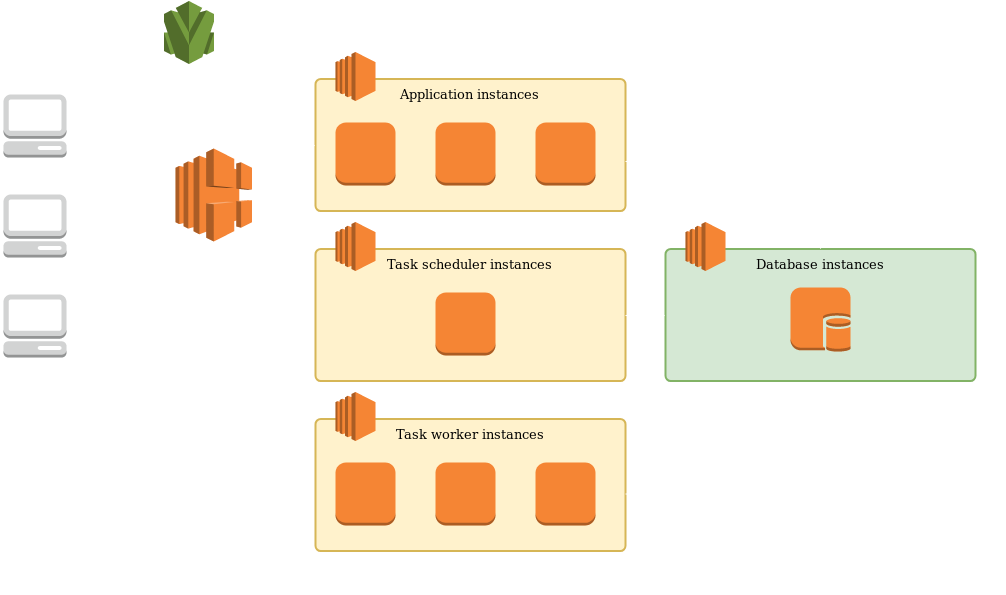
\includegraphics[width=8cm]{images/opsworks_diagram.png}
  \end{frame}

  \begin{frame}{GAT infrastructure}
  \framesubtitle{Pain points explained}
  \begin{itemize}
    \item Long deployment times
    \item Uncertainty of success before starting
    \item Deployments caused downtime
    \item High cost
    \item Not automated
  \end{itemize}
  \end{frame}

  % ---------------------------------- %

  \imageframe{images/container_landscape.jpg}{The container landscape}

  \begin{frame}{Docker}
    \begin{columns}[c]
      \begin{column}{.3\textwidth}
          
\includegraphics[width=3cm,height=3cm]{images/docker_logo.png}
      \end{column}
      \begin{column}{.7\textwidth}
        \begin{itemize}
          \item Container platform
          \item Lightweight virtual machines
          \item Packaging format
        \end{itemize}
      \end{column}
    \end{columns}
  \end{frame}

  \begin{frame}{Kubernetes}
    \begin{columns}[c]
      \begin{column}{.3\textwidth}
          
\includegraphics[width=3cm,height=3cm]{images/kubernetes_logo.png}
      \end{column}
      \begin{column}{.7\textwidth}
        \begin{itemize}
          \item Container orchestration
          \item Service discovery
          \item Persistent storage
          \item High availability
        \end{itemize}
      \end{column}
    \end{columns}
  \end{frame}

  \begin{frame}{Helm}
    \begin{columns}[c]
      \begin{column}{.3\textwidth}
          
\includegraphics[width=3cm,height=3cm]{images/helm_logo.png}
      \end{column}
      \begin{column}{.7\textwidth}
        \begin{itemize}
          \item Package manager for Kubernetes
          \item Configuration management
          \item Deployment management
          \item Template provider
        \end{itemize}
      \end{column}
    \end{columns}
  \end{frame}

  % ---------------------------------- %

  \imageframe{images/migrating_cranes.jpg}{Migrating to Kubernetes}

  \begin{frame}{Moving to Kubernetes on GKE}
  \framesubtitle{Why there?}
  \begin{itemize}
    \item Cluster deployment is completely automated
    \item Management is done by Google
    \item Built in goodies
    \begin{itemize}
      \item Authentication integrated with the rest of their cloud
      \item Centralized logging
      \item Cluster monitoring
      \item Container registry
    \end{itemize}
  \end{itemize}
  \end{frame}

  \begin{frame}{Moving to Kubernetes on GKE}
  \framesubtitle{The journey}
  \begin{itemize}
    \item Docker images for applications
    \item CI pipeline modification
    \item Helm charts to replace the currently used automation
    \item Moving the apps one by one
    \begin{itemize}
      \item First on sandbox environments
      \item No weird dependencies, only API communication
    \end{itemize}
  \end{itemize}
  \end{frame}

  \begin{frame}{Moving to Kubernetes on GKE}
  \framesubtitle{The end result}
  \centering
  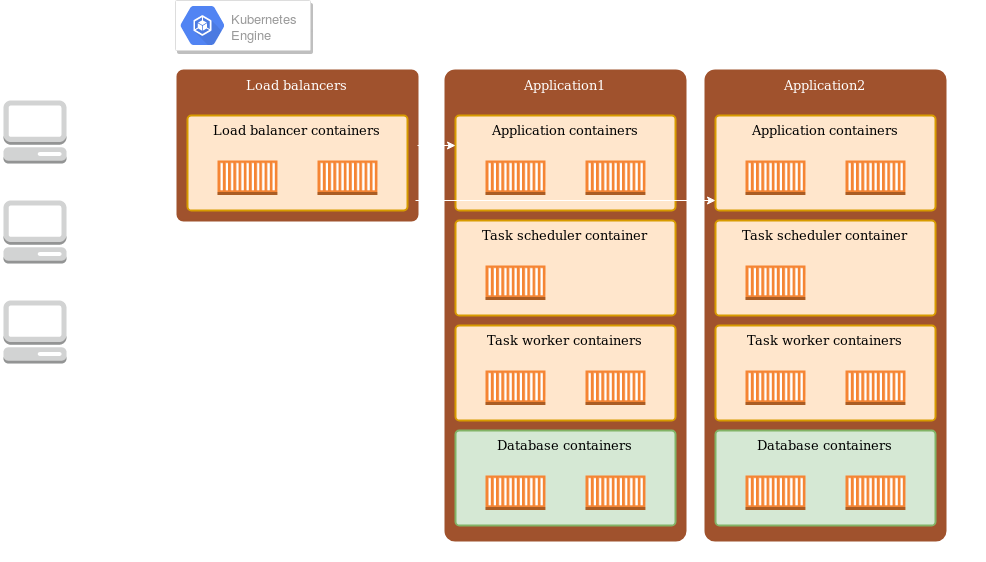
\includegraphics[width=8cm]{images/kubernetes_diagram.png}
%  \begin{itemize}
%    \item TODO: Diagram goes here
%    \item Deployment flow unchanged
%    \item Basic architecture stays the same
%  \end{itemize}
  \end{frame}

  \begin{frame}{Moving to Kubernetes on GKE}
  \framesubtitle{No happy end}
  \begin{itemize}
    \item Bugs!
    \begin{itemize}
      \item Nodes crashing due to misconfigured journalctl
      \item Frequent networking problems
    \end{itemize}
    \item Management is done by Google
    \begin{itemize}
      \item Forced, automatic security updates on master nodes
      \item No way of accessing the machine
      \item Doesn't work? Too bad
    \end{itemize}
    \item Inflexible configuration
    \begin{itemize}
      \item Not possible to turn on alpha features
      \item Not possible to change node configuration
      \item Even pulling an image before attaching a~node to the cluster is hard
    \end{itemize}
  \item Waiting for Kubernetes security updates (CVE-2017-1002101 and it's 4 days)
  \end{itemize}
  \end{frame}

  \begin{frame}{Moving to Kubernetes on AWS}
  \framesubtitle{Enter kops}
  \begin{itemize}
    \item A~Kubernetes cluster bootstrapping utility
  \end{itemize}
  \end{frame}

  \begin{frame}{Moving to Kubernetes on AWS}
  \framesubtitle{New challenges}
  \begin{itemize}
    \item Missing parts
    \begin{itemize}
      \item Authentication integrated with the rest of their cloud - \textbf{PKI}
      \item Centralized logging - \textbf{Graylog}
      \item Cluster monitoring - \textbf{Prometheus and Grafana}
    \end{itemize}
    \item Moving stuff
    \begin{itemize}
      \item Container registry - \textbf{Amazon ECR}
      \item AWS and GKE load balancers behave differently
      \item Use EBS instead of Google disks
    \end{itemize}
  \end{itemize}
  \end{frame}

  \imageframe{images/questions.jpg}{Questions?}

\end{document}
